% Created 2019-01-17 Thu 09:18
% Intended LaTeX compiler: pdflatex
\documentclass[t, aspectratio=169, allowframebreaks]{beamer}
\usepackage[utf8]{inputenc}
\usepackage[T1]{fontenc}
\usepackage{graphicx}
\usepackage{grffile}
\usepackage{longtable}
\usepackage{wrapfig}
\usepackage{rotating}
\usepackage[normalem]{ulem}
\usepackage{amsmath}
\usepackage{textcomp}
\usepackage{amssymb}
\usepackage{capt-of}
\usepackage{hyperref}
\usepackage{minted}
\beamertemplatenavigationsymbolsempty
\usepackage[numbers, authoryear, round]{natbib}
\BeforeBeginEnvironment{frame}{\subsection{}}
\usetheme[compress]{Amsterdam}
\author{Nathan Hughes}
\date{\today}
\title{How do \emph{cis}-regulatory elements evolve in plants?}
\hypersetup{
 pdfauthor={Nathan Hughes},
 pdftitle={How do \emph{cis}-regulatory elements evolve in plants?},
 pdfkeywords={},
 pdfsubject={},
 pdfcreator={Emacs 26.1 (Org mode 9.1.9)},
 pdflang={English}}
\begin{document}

\maketitle
\begin{frame}{Outline}
\tableofcontents
\end{frame}

\let\tempone\itemize
\let\temptwo\enditemize
\renewenvironment{itemize}{\tempone\addtolength{\itemsep}{0.6\baselineskip}}{\temptwo}

\addtobeamertemplate{block begin}{%
  \setlength{\textwidth}{1.0\textwidth}%
}{}

\addtobeamertemplate{block alerted begin}{%
  \setlength{\textwidth}{1.0\textwidth}%
}{}

\addtobeamertemplate{block example begin}{%
  \setlength{\textwidth}{1.0\textwidth}%
}{}


\setbeamerfont{caption}{size=\footnotesize}

\setbeamertemplate{caption}[numbered]
\setbeamerfont{bibliography item}{size=\footnotesize}
\setbeamerfont{bibliography entry author}{size=\footnotesize}
\setbeamerfont{bibliography entry title}{size=\footnotesize}
\setbeamerfont{bibliography entry location}{size=\footnotesize}
\setbeamerfont{bibliography entry note}{size=\footnotesize}
\setbeamertemplate{bibliography item}{\insertbiblabel}



\section{Introduction}
\label{sec:org4e35c5a}
\begin{frame}[label={sec:orge90f659}]{What is the project?}
\begin{block}{\alert{Main question}: How do \emph{cis}-regulatory elements evolve in plants?}
\begin{itemize}
\item \emph{Cis} meaning same
\begin{itemize}
\item in this case elements on the same DNA strand
\end{itemize}
\item i.e. how do non-coding elements on the same DNA strand affect gene expression?
\end{itemize}
\end{block}
\end{frame}

\begin{frame}[label={sec:org8ff550c}]{What are \emph{cis}-regulatory elements?}
\begin{block}{\emph{Cis}-regulatory elements}
\begin{itemize}
\item They are usually enhancers and promoters that control development and physiology by regulating gene expression. \footnote{\cite{wittkoppCisregulatoryElementsMolecular2012}}
\end{itemize}

\begin{figure}[htbp]
\centering
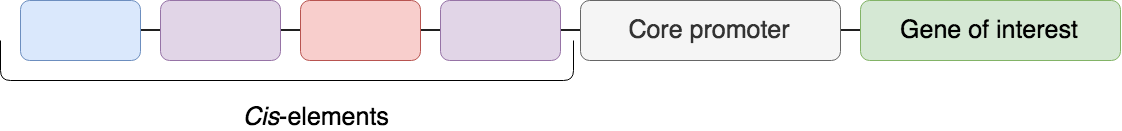
\includegraphics[width=9cm]{./cis-elements.png}
\caption{\label{fig:orgfe20d23}
Example promoter containing cis-regulatory elements. Cis-elements can be repeated more than once (purple) and can recruit different transcription factors (blue/red), all driving the same gene (green)}
\end{figure}
\end{block}
\end{frame}

\begin{frame}[label={sec:org92ca40e}]{Why are they important?}
\begin{block}{Gene expression / phenotypic variation}
\begin{itemize}
\item For most of the twentieth century, evolution of protein-coding sequences was commonly thought to be primarily (if not solely) responsible for phenotypic evolution
\item Whereas more recent studies show that mutations which affect the function of these sequences contribute to phenotypic diversity within and between species
\begin{itemize}
\item Many studies imply divergent \emph{cis}-regulatory activity in phenotypic evolution \footnote{\cite{carrollEvoDevoExpandingEvolutionary2008}}
\end{itemize}
\end{itemize}
\end{block}
\end{frame}

\section{Methods}
\label{sec:orgc899a07}

\begin{frame}[label={sec:orgf0ff41c}]{How can you study the evolution of \emph{cis}-regulatory elements, in plants?}
\begin{columns}
\begin{column}{0.5\columnwidth}
\begin{block}{Materials}
\begin{itemize}
\item Start with a little known plant: \emph{Arabidopsis thaliana}
\begin{itemize}
\item Has an extremely well covered genome, as well as transcription factor database
\end{itemize}
\item Will later move towards \emph{Nicotiana benthamiana}, to evaluate how transferable work on model systems are to others'
\end{itemize}
\end{block}
\end{column}

\begin{column}{0.5\columnwidth}
\begin{block}{Plants}
\begin{figure}[htbp]
\centering
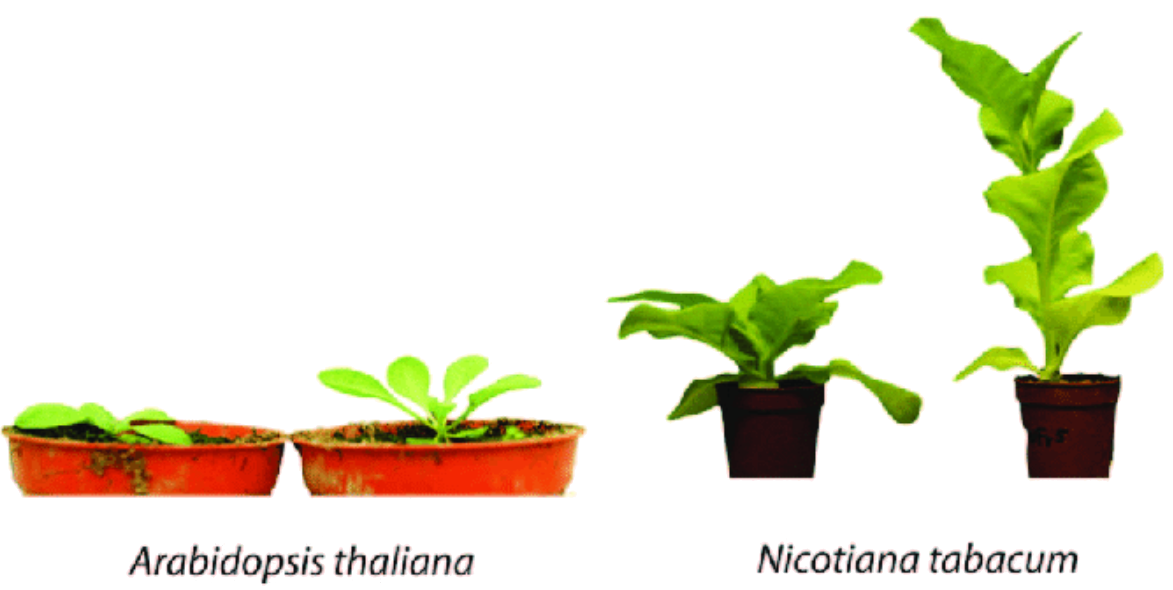
\includegraphics[width=6.4cm]{./plants.png}
\caption{\label{fig:org0024819}
Example of \emph{Arabidopsis} and \emph{Nicotiana}}
\end{figure}
\end{block}
\end{column}
\end{columns}
\end{frame}

\begin{frame}[label={sec:org2e03c79}]{Promoter study}
\begin{block}{Procedure to evaluate ?}
First choose two types of promoters to study:

\alert{The most constitutively expressed} and \alert{Nitrogen-responsive}

For each promoter type:
\begin{enumerate}
\item Identify motifs where TFs bind, check if any TFs are commonly used
\item Determine whether any patterns or similarities are present in groups/types of TFs
\item Incorporate nucleosome occupancy data (whether DNA is wrapped around a nucleosome or is open)
\item Verify hypothesis in lab
\end{enumerate}
\end{block}
\end{frame}


\section{Progress}
\label{sec:org6288a3f}

\begin{frame}[label={sec:orged2d939}]{Identifying TF binding motifs of interest}
\begin{block}{Using MEME and FIMO to predict TF binding motifs}
\begin{figure}[htbp]
\centering
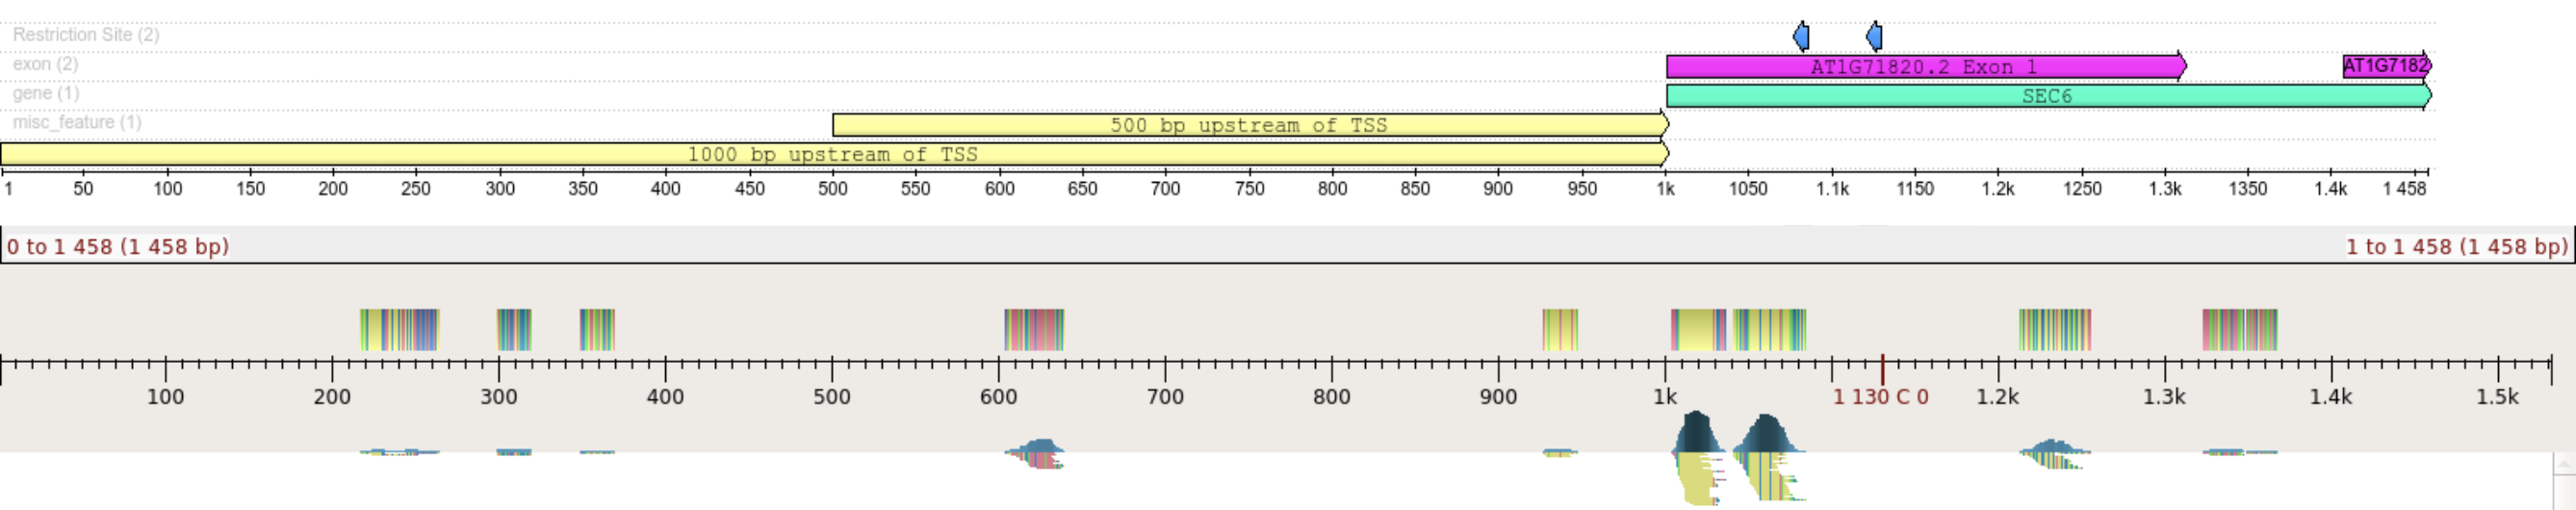
\includegraphics[width=14cm]{./genes.png}
\caption{\label{fig:org0ae49aa}
Example FIMO output for promoter of AT1G71820}
\end{figure}
\end{block}
\end{frame}

\begin{frame}[label={sec:org5450446}]{Lab work}
\begin{block}{Progress towards testing selected regions of interest}
\begin{itemize}
\item Designed primers in Benchling and ordered them for each of the promoters/promoter parts if mutating RE cut site
\item Ran PCR with primers and At template DNA
\begin{itemize}
\item didn't work, changed conditions
\item tried different DNA template - worked
\end{itemize}
\item Made own At CTAB DNA template
\begin{itemize}
\item PCR didn’t work
\end{itemize}
\item Using higher concentration of template DNA worked
\end{itemize}
\end{block}
\end{frame}


\begin{frame}[allowframebreaks,label=]{References}
\bibliographystyle{unsrtnat}
\bibliography{../../Notes/library}
\end{frame}
\end{document}